\section{Experiments}
Leis et al. recently argued for improved benchmarks for evaluating join ordering algorithms, and proposed the ``Join Order Benchmark'' (JOB)~\cite{leis2015good}.
This benchmark is derived from the Internet Movie Data Base
(IMDB). It contains information
about movies and related facts about actors, directors,
production companies, etc. 
The dataset is 3.6 GB in size and consists of 21 relational tables.
The largest table has
36 million rows.
The benchmark contains 33 queries which have between 5 and 15 joins, with an average of 8 joins per query.  
We evaluate \sys on this benchmark in terms of planning latency and plan cost.


\subsection{JOB Cost Models}
As a secondary contribution of this paper, we find that the particular choice of cost model and physical design greatly affects results.
The same query with different cost models can lead to different top-performing heuristics.
Crucially, we find that many heuristics are sensitive to non-linearities.

The cost model described in~\cite{leis2015good} is inspired by an in-memory system. The cost of a hash join is linear in the size of the input relations, and the cost of an index join is essentially the cost of streaming the left side of the join.
This cost model greatly rewards index-usage (by convention the right relation is used for index lookup), and left-deep strategies are very strong in this setting. In fact, the authors claim: 
\begin{quote}
\emph{``The bad performance of right-deep trees is caused by the large intermediate hash tables that need to be created from each base relation and the fact that only the bottom-most join can
be done via index lookup.''}~\cite{leis2015good} 
\end{quote}
The conclusion is that the marginal benefit of bushy plans is small compared to the additional search costs.
We argue that this is a consequence of the cost model and physical design and this led us to explore alternative cost models where the left-deep heuristic might fail.

\vspace{0.25em} \noindent \textbf{CM1: } In the first cost model (inspired by~\cite{leis2015good}), we model a main-memory database that performs two types of joins: index nested-loop joins and in-memory hash joins. Let $O_l$ be the left operator and $O_r$ be the right operator. The costs are defined as follows:
\[
\textsf{c}_{inlj} = \textsf{c}(O_l) + \textsf{rf}(O_l, O_r) \cdot |O_l|
\]
\[
\textsf{c}_{hj} = \textsf{c}(O_l) + \textsf{c}(O_r)
\]
where \textsf{c} denotes the cost estimation function and \textsf{rf} denotes the estimated reduction factor of the join.
As we can see, this model favors index-based joins when available. 
The reduction factor $\textsf{rf}(O_l, O_r)$ is always less than 1.
More importantly, this cost model is a justification for the use of left-deep plans.
In $\textsf{c}_{inlj}$, the right operator does not incur a scan cost.
A left deep tree where the indexed relations are on the right exploits this structure. We include primary key and foreign indexes on all relations.


\vspace{0.25em} \noindent \textbf{CM2: } In the next cost model, we model a database that accounts for disk-memory relationships in the hash joins. We designate the left operator as the ``build'' operator and the right operator as the ``probe'' operator. 
If the previous join has already built a hash table on an attribute of interest, then the hash join does not incur another cost.
\[
\textsf{c}_{nobuild} = \textsf{c}(O_r)
\]
This model favors right-deep plans which maximize the reuse of the built hash tables.


\vspace{0.25em} \noindent \textbf{CM3: } Finally, in the next cost model, we model temporary tables and memory capacity constraints. There is a budget of tuples that can fit in memory and an additional physical operator that allows for materialization of a join result if memory exists. Then, the downstream cost of reading from a materialized operator is 0.   
\[
\textsf{c}(O) = 0 \text{ if materialized}
\]
This model requires bushy plans due to the inherent non-linearity of the cost function and memory constraints. 
The cost model encourages plans that group tables together in ways that the join output can fit in the available memory.

\vspace{0.5em} In our implementation of these cost models, we use \emph{true} cardinalities on single table predicates and two-way joins of base relations. We leverage standard independence assumptions to construct more complicated cardinality estimates. The goal of this work is to evaluate the join ordering process independent of the strength or weakness of the underlying cardinality estimation. 

\subsection{Baseline Algorithms}
We consider the following baseline algorithms. These algorithms are not meant to be a comprehensive list of heuristics but rather representative of a class of solutions.

\begin{enumerate}
    \item Exhaustive (\textbf{EX}): This is a dynamic program that exhaustively enumerates all join plans avoiding cartesian products.
    \item Left-Deep (\textbf{LD}): This is a dynamic program that exhaustively enumerates all left-deep join plans.
    \item Right-Deep (\textbf{RD}): This is a dynamic program that exhaustively enumerates all right-deep join plans.
    \item Zig-Zag (\textbf{ZZ}): This is a dynamic program that exhaustively enumerates all zig-zag trees that is every join has at least one base relation (either on the left or the right).
    \item IK-KBZ (\textbf{KBZ}): This algorithm is a polynomial time approximation that decomposes the query graph into chains and orders the chains based on a linear approximation.
    \item QuickPick-1000 (\textbf{QP}): This algorithm randomly selects 1000 joins and returns the best of them. 1000 was selected to be roughly equivalent to the planning latency of \sys.
\end{enumerate}

\subsection{Optimizer Cost}
In the first experiment, we evaluate all of the baseline algorithms against \sys in terms of final optimization cost. All of the algorithms consider join ordering without cartesian products, so \textbf{EX} is a baseline optimal solution. We report results in terms of the suboptimality w.r.t \textbf{EX}.

\subsubsection{Without Single Table Selections}
We first evaluate consider the 33 join order benchmark query templates without single table selections. We train on 26 queries and test on 7 held out queries. We report results averaged over 5-fold cross-validation (so all of the reported numbers are when the query is not seen during training). We report the min, mean, and max cost relative to the baseline.  For randomized algorithms the max range of performance (as a multiplicative factor) over 5 trials.

In the first experiment, we consider CM1. This is an idealized model that heavily encourages index usage. All of the optimal plans for this workload are left-deep. Predictably, right-deep plans perform very poorly. \sys significantly out performs the heuristic solutions \textbf{KBZ} and \textbf{QP}. \sys is also far more reliable in terms worst case performance. 

\begin{table}[ht!]\centering \small
\caption{CM1 No Selections. Cost Relative to Optimal Plan. }\vspace{0.25em}
\begin{tabular}{|l|l|l|l|l|}
\hline
    & {\bf Min}  & {\bf Mean}  & {\bf Max}    & {\bf Range-Max} \\ \hline
{\bf QP}  & 1.0  & 23.87 & 405.04 & 2.11x      \\ \hline
{\bf KBZ} & 1.0  & 3.45  & 36.78  & -         \\ \hline
{\bf RD}  & 4.70 & 53.25 & 683.35 & -         \\ \hline
{\bf LD}  & 1.0  & 1.0   & 1.0    &           \\ \hline
{\bf ZZ}  & 1.0  & 1.0   & 1.0    & -         \\ \hline
{\bf EX}  & 1.0  & 1.0   & 1.0    & -         \\ \hline
\hline
{\bf DQ}  & 1.0  & 1.36   & 3.11    & 1.79x\\ \hline
\end{tabular}
\end{table}

By simply changing the cost model, we can force exactly the opposite heuristic to perform well. When we evaluate CM2, which accounts for reuse of hash tables, right-deep plans are no longer so poor. In this cost model, none of the heuristics match the exhaustive search over the entire workload. \sys comes close and it is actually significantly better than zig-zag enumeration for this cost model.

\begin{table}[ht!]\centering \small
\caption{CM2 No Selections. Cost Relative to Optimal Plan. }\vspace{0.25em}
\begin{tabular}{|l|l|l|l|l|}
\hline
    & {\bf Min}  & {\bf Mean}  & {\bf Max}    & {\bf Range-Max} \\ \hline
{\bf QP}  & 1.43  & 16.74 & 211.13 & 1.71x      \\ \hline
{\bf KBZ} & 2.21  & 14.61  & 96.14  & -         \\ \hline
{\bf RD}  & 1.83 & 4.25 & 69.15 & -         \\ \hline
{\bf LD}  & 1.35  & 5.21   & 55.45    &           \\ \hline
{\bf ZZ}  & 1.0  & 3.41   & 23.13    & -         \\ \hline
{\bf EX}  & 1.0  & 1.0   & 1.0    & -         \\ \hline
\hline
{\bf DQ}  & 1.0  & 1.91   & 13.14    & 1.43x\\ \hline
\end{tabular}
\end{table}

CM3 is meant to illustrate a cost-model where no heuristic performs well. We count the number of tuples materialized and to benfit from the materialization these tuples must fit into memory. This leads to a ``packing'' like optimization problem where the exact join order also depends on how well the intermediate results can be packed into memory. \sys is still performant in this setting as it adapts to the properties of the workload.

\begin{table}[ht!]\centering \small
\caption{CM3 No Selections. Cost Relative to Optimal Plan. }\vspace{0.25em}
\begin{tabular}{|l|l|l|l|l|}
\hline
    & {\bf Min}  & {\bf Mean}  & {\bf Max}    & {\bf Range-Max} \\ \hline
{\bf QP}  & 1.78  & 46.19 & 489.13 & 3.44x      \\ \hline
{\bf KBZ} & 1.21  & 56.44  & 296.14  & -         \\ \hline
{\bf RD}  & 4.41 & 87.25 & 369.97 & -         \\ \hline
{\bf LD}  & 1.21  & 49.32   & 255.60    &           \\ \hline
{\bf ZZ}  & 1.16  & 21.44   & 243.16    & -         \\ \hline
{\bf EX}  & 1.0  & 1.0   & 1.0    & -         \\ \hline
\hline
{\bf DQ}  & 1.0  & 3.76   & 113.89    & 2.51x\\ \hline
\end{tabular}
\end{table}

\vspace{0.5em}\noindent \textbf{Summary and Caveats: }  We showed that heuristics are often myopic and can perform very poorly when the problem structure changes. A learning-based approach can adapt to the different scenarios at the cost of training data. As a caveat, we used idealized cost models with true cardinality values to evaluate the performance of different optimization and pruning heuristics. The experiment is meant to illustrate the mathematical structure of the optimization problem and does not make a claim about execution performance or plan variance.

\subsubsection{With Single Table Selections}
Next, we show the performance of \sys on the 113 JOB queries when we include single table selections. The point of this experiment is to illustrate an interesting difference between learning-based and enumeration-based optimization. When true cardinalities are available, single table selections are not a problem for classical optimizers, but a learning optimizer has to correlate reduction factors with changes in join decisions. This is difficult without observing a lot of different predicates at a variety of selectivities.
It is easy to generate a large dataset with a lot of different join orders, however, generating random predicates on the tables can be more challenging. We train on 80 queries and test on 33 queries. We do 4 fold cross validation to ensure that every test query is excluded from the training set at least once. 

\begin{table}[ht!]\centering \small
\caption{Effect of Single Table Selections on \sys }\vspace{0.25em}
\begin{tabular}{|l|l|l|l|l|}\hline
    & {\bf Min}  & {\bf Mean}  & {\bf Max}    & {\bf Range-Max} \\ \hline
{\bf CM1. No Sel}  & 1.0  & 1.36   & 3.11    & 1.79x\\ \hline
{\bf CM1. Sel}  & 1.0  & 2.14   & 8.43    & 2.86x\\ \hline
{\bf CM2. No Sel}  & 1.0  & 1.91   & 13.14    & 1.43x\\ \hline
{\bf CM2. Sel}  & 1.0  & 3.55   & 38.54    & 1.96x\\ \hline
{\bf CM3. No Sel}  & 1.0  & 3.76   & 113.89    & 2.51x\\ \hline
{\bf CM3. Sel}  & 1.0  & 6.44   & 207.09    & 3.56x\\ \hline
\end{tabular}
\end{table}

One approach addressing this issue is to augment the dataset with synthetic predicates. We could randomly sample equality conditions on each of the single tables. Figure \ref{exp:plot1} illustrates the results. We augment our training workload with a 100 additional training queries with random single table selections. With this data, we can better attribute the effects of selection on costs.   

\begin{figure}
    \centering
    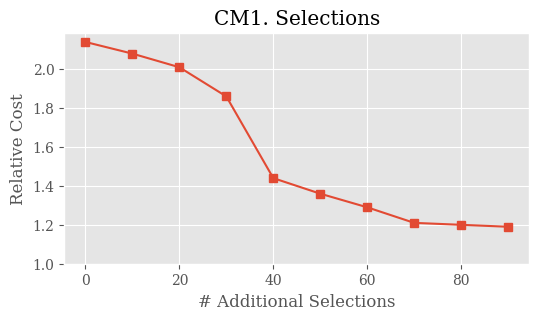
\includegraphics[width=0.8\columnwidth]{exp/exp1_plot1.png}
    \caption{Accurately modeling the effects of single table selections requires more training data. Generating a modest number of synthetic single table equality predicates can help. We plot the mean relative cost of \sys as a function of the number of synthetic predicates. \label{exp:plot1}}
\end{figure}

Selections are interesting because they have threshold effects on cost. Once a selectivity of a predicate on one of the relations drops beyond a certain point--the set of low cost plans might drastically change. These results are both positive and negative. First, it illustrates that learning-based approaches can easily be made robust to different phenomena by manipulating the training data and/or the featurization. On the other hand, the system may not accurately be able to assess its own confidence on previously unseen plans. It might make predictions assuming smooth behavior without knowledge of a drastic change due to selectivity. 

\subsection{Data Quantity/Quality}
We further evaluate the nature of training data required by \sys, in terms of raw quantity (number of training queries seen) and quality (the relevance to the test workload).

\subsubsection{Quantity}
We consider the optimization with no single table selections and use CM1. We vary the number of training queries given to \sys and plot the mean relative cost to optimal. Figure \ref{exp:plot2} illustrate the relationship. \sys requires about 30 training queries to match the performance of QuickPick 1000.

\begin{figure}
    \centering
    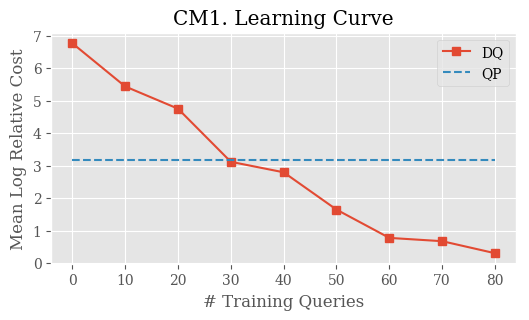
\includegraphics[width=0.8\columnwidth]{exp/exp2_plot1.png}
    \caption{The mean relative cost as a function of the number of training queries to \sys. We include QuickPick as a baseline. \label{exp:plot2}}
\end{figure}

We found that this break even point roughly corresponds to seeing all of the relations in a query at least once. In fact, one can train the model on ``small queries'' and test it on larger ones--as long as the relations are covered well. We trained \sys on all of the queries with less than 9 relations and tested on the remaining queries. Similarly, we trained on all of the queries with less than 8 relations and tested on the remaining queries. 

\begin{table}[ht!]\centering \small
\caption{Effect of Single Table Selections on \sys }\vspace{0.25em}
\begin{tabular}{|l|l|l|l|l|}\hline
    & {\bf Min}  & {\bf Mean}  & {\bf Max}    & {\bf Range-Max} \\ \hline
{\bf Random}  & 1.0  & 1.36   & 3.11    & 1.79x\\ \hline
{\bf Train} $< 9$  & 1.0  & 2.09   & 11.11    & 1.64x\\ \hline
{\bf Train} $< 8$  & 1.0  & 9.91   & 53.66    & 2.43x\\ \hline
\end{tabular}
\end{table}

Even when trained on subplans, \sys performs relatively well. This indicates that the structure that \sys is learning is local---how combinations of relations join together efficiently.

\subsubsection{Relevance of Training Data}
Next, we consider the effect of different training data sampling schemes. 
We consider the optimization with single table selections and use CM1.
Figure \ref{exp:plot3} plots the performance of different data sampling techniques each with 80 training queries. The more relevant the training queries can be made towards the test workload, the less data is required for good performance.

\begin{figure}
    \centering
    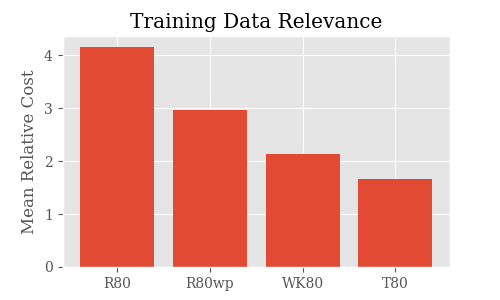
\includegraphics[width=0.8\columnwidth]{exp/exp2_plot2.png}
    \caption{We plot the relative performance of \sys with different training workloads. R80 is a dataset sampled independent of the JOB workload with random joins from the schema and random equality predicates. R80wp is samples from random joins as before but single table predicates from the workload. WK 80 includes 80 queries samples from the workload, and T80 describes a scheme where each of the 33 query templates is covered at least once in sampling. \label{exp:plot3}}
\end{figure}

It also shows that the performance does not completely suffer with random queries. 
\sys still achieves a lower cost compared to Quick Pick 1000 even with random queries.
The goal of this experiment is to illustrate that \sys does not actually require \emph{a priori} knowledge of the workload.

\subsubsection{Quality of Training Planner}
Next, we evaluate different training planners for collecting the training dataset.  We consider the optimization with single table selections and use CM1. We collect a varying amount of data sampled from queries in the workload. We compare using a QuickPick 1000 planner, Left-Deep planner, and the Bushy planner described earlier (Figure \ref{exp:plot4}).  All of the methods very quickly converge to good solutions. The dynamic programming-based methods, Left-Deep and Bushy, converge faster as they generate training data for subplans as well. The QuickPick planner gives us 1000 random trajectories per query.
The subplan structure is very valuable for training and covering the space of different relation combinations that might be seen in testing.


\begin{figure}
    \centering
    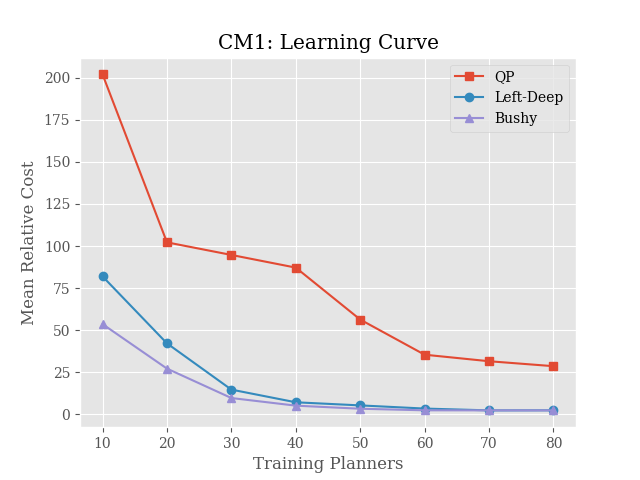
\includegraphics[width=0.8\columnwidth]{exp/exp2_plot3.png}
    \caption{ We compare using a QuickPick 1000 planner, Left-Deep planner, and the Bushy planner to collect training data.\label{exp:plot4}}
\end{figure}


\subsubsection{Model Choice}
In theory, with enough data, \sys should be approaching optimal performance.
The natural next question is where does the gap come from---is it the neural networks ability to represent the cost function (Model-Limited) or is it a lack of training data (Data-Limited).
We ran an experiment on the first 20 training queries. \sys sees these queries in training as well as during testing. This measures the ability to memorize training data. We train the model to convergence and measure the error. We report the fraction of 20 queries where the learned planner exactly matched the optimal planner performance.

\begin{table}[ht!]\centering \small
\caption{Ability to Memorize}\vspace{0.25em}
\begin{tabular}{|l|l|l|l|}\hline
    & {\bf CM 1}  & {\bf CM 2}  & {\bf CM 3} \\ \hline
{\bf With Selections}  & 0.90  & 0.75   & 0.90 \\ \hline
{\bf Without Selections}  & 1.0  & 0.80   &  0.95\\ \hline
\end{tabular}
\end{table}

We see that there is some inherent imprecision in the neural network, even if the exact testing query has been seen before. We find that this has less to do with the linearity or non-linearity of the cost function, but rather how ``close'' good plans are in terms of cost. If there are a lot of roughly similar good plans the neural network may not have enough precision to differentiate between them.
This means that even with unlimited data we may not match an optimal planner. 

This does raise the question about our modeling choices. We do an ablation study of the featurization choices described in the paper and they really suggest that all of the different features are necessary for performance:

\begin{table}[ht!]\centering \small
\caption{Feature Ablation}\vspace{0.25em}
\begin{tabular}{|l|l|l|l|}\hline
    & {\bf Graph Features}  & {\bf Sel. Scaling}  & {\bf Loss} \\ \hline
{\bf No Selections}  & N  & N   & 0.087 \\ \hline
 & Y  & N   & 0.04914 \\ \hline
  & Y  & Y   & 0.04914 \\ \hline
\hline
{\bf Selections}  & N  & N   &  0.071\\ \hline
& Y  & N   &  0.051\\ \hline
& Y  & N   &  0.020\\ \hline
\end{tabular}
\end{table}

Without features derived from the query graph and scaling based on the cost model the training loss is 3.5x more. This means that the network cannot predict accurately even on the training data.

\subsubsection{Sensitivity Analysis}
\textbf{TODO}

\subsection{Runtime}
\textbf{TODO}

\subsection{Real Execution}
\textbf{TODO}

